%\documentclass[sigconf,anonymous]{llncs}
%\documentclass[9pt]{IEEEtran}
\documentclass[twocolumn]{svjour3}
\usepackage{amsmath}
\usepackage{amsfonts}
\usepackage{hyperref}
\usepackage{epstopdf}
%\usepackage{subcaption}
\usepackage{csquotes}
\usepackage[toc,section=chapter]{glossaries}
\usepackage{acronym}
\usepackage{yfonts}
\usepackage{listings}

\usepackage{pdfpages}
\usepackage{mwe}
\usepackage{pgfplots}
\usepackage{tikz}
\usepackage{caption}
\usepackage{pgfplotstable}
\usepackage{float}
\usepackage{multirow}


\usepackage{algorithm}
%\usepackage{algorithmic}
\usepackage{algpseudocode}
\usepackage[ruled, vlined, linesnumbered,algo2e,]{algorithm2e}
\usepackage{booktabs}
\usepackage[font=small,labelfont=bf]{caption}
\usepackage{tikz-timing}
\usetikztiminglibrary[rising arrows]{clockarrows}
\usetikzlibrary{positioning,patterns}

\usepackage{graphicx}
\usepackage{hhline}

\usepackage{tabularx}


\usepackage{numprint}
\npdecimalsign{.}
\npthousandsep{,}

\usepackage{array,multirow,graphicx}
\usepackage{float}

\newcommand\Tstrut{\rule{0pt}{2.5ex}}    % = `top' strut
\newcommand\Bstrut{\rule[-1ex]{0pt}{0pt}}   % = `bottom' strut

\newcommand{\mailtodomain}[1]{\href{mailto:#1@bristol.ac.uk}{\nolinkurl{#1}}}
\usepackage{etoolbox}

\newcolumntype{x}[1]{>{\centering\let\newline\\\arraybackslash\hspace{0pt}}p{#1}}
\newcolumntype{y}[1]{>{\raggedright\let\newline\\\arraybackslash\hspace{0pt}}p{#1}}
\newcolumntype{z}[1]{>{\raggedleft\let\newline\\\arraybackslash\hspace{0pt}}p{#1}}

\usepackage{adjustbox}
\usepackage{booktabs}

\newcolumntype{R}[2]{%
    >{\adjustbox{angle=#1,lap=\width-(#2)}\bgroup}%
    l%
    <{\egroup}%
}
\newcommand*\rot{\multicolumn{1}{R{90}{-0.251em}}}% no optional argument here, please!


\begin{document}

%\title{Optimised Lattice-Based Key Encapsulation in Hardware}
\title{A Design Space Exploration for Optimizing Lattice-Based Key Encapsulation in Hardware}
%
%\author{\IEEEauthorblockN{James Howe}\textsuperscript{$\ast$}, \IEEEauthorblockN{Marco Martinoli}\textsuperscript{$\dagger$}, \IEEEauthorblockN{Elisabeth Oswald}\textsuperscript{$\ddagger$}, and \IEEEauthorblockN{Francesco Regazzoni}\textsuperscript{$\dagger$} \\
%\IEEEauthorblockA{\textsuperscript{$\ast$}{PQShield Ltd.}, Oxford, United Kingdom.\\ {\href{mailto:james.howe@pqshield.com}{james.howe@pqshield.com}}} \\
%\IEEEauthorblockA{\textsuperscript{$\dagger$}{Department of Computer Science}, {University of Bristol}, Bristol, UK. \\
%\{\href{mailto:marco.martinoli@bristol.ac.uk}{marco.martinoli}, \href{mailto:elisabeth.oswald@bristol.ac.uk}{elisabeth.oswald}\}@bristol.ac.uk }\\
%\IEEEauthorblockA{\textsuperscript{$\ddagger$}{Advanced Learning and Research Institute}, {Universit\`{a} della Svizzera Italiana}, Switzerland.\\ \href{mailto:regazzoni@alari.ch}{regazzoni@alari.ch} }
%}

%\{marco.martinoli,elisabeth.oswald\}@bristol.ac.uk} \\
%\mailtodomain{\{marco.martinoli, elisabeth.oswald\}}@bristol.ac.uk} \\

\author{%
%James Howe\inst{1}  \and 
%Marco Martinoli\inst{2} \and
%Elisabeth Oswald\inst{2} \and 
%Francesco Regazzoni\inst{3}
%}%
%\institute{
%PQShield Ltd., Oxford, United Kingdom\\
%\email{james.howe@pqshield.com},\\ 
%\and
%Department of Computer Science, University of Bristol, United Kingdom\\
%\texttt{\{marco.martinoli,elisabeth.oswald\}@bristol.ac.uk}\\
%\and
%Advanced Learning and Research Institute, Universit\`{a} della Svizzera Italiana, Switzerland\\
%\email{regazzoni@alari.ch}
Anonymous
}

\maketitle
\begin{abstract} \label{astract}
%FrodoKEM is a lattice-based key encapsulation mechanism, currently a semi-finalist in NIST’s post-quantum standardization effort. Most candidates utilize a NIST standard for randomness, a SHA-3 variant, however this is a significant implementation bottleneck. Trivium is a lightweight, ISO standard designed for hardware, having been used in previous implementation of lattice-based cryptography. This research proposes optimized designs for FrodoKEM, concentrating on high-throughput by parallelising its time-consuming matrix multiplication operations. The parallelisations proposed also complement the addition of first-order masking to decapsulation. We significantly increase \newline FrodoKEM’s throughput; with a $\sim$16x speed-up compared to the previous state-of-the-art, whilst also maintaining a similar FPGA area footprint.

FrodoKEM is a lattice-based key encapsulation mechanism, currently a semi-finalist in NIST’s post-quantum standardization effort. A condition for these candidates is to use NIST standards for PRNG /
seed-expanding, and as such most candidates utilize SHAKE, an XOF defined in the SHA-3 standard. However, for many of the candidates, this module is a significant implementation bottleneck. Trivium is a lightweight, ISO standard stream cipher which performs well in hardware and has been used in previous hardware designs for lattice-based cryptography. This research proposes optimized designs for FrodoKEM, concentrating on high throughput by parallelising the matrix multiplication operations within the cryptographic scheme. This process is eased by the use of Trivium due to its higher throughput and lower area consumption. The parallelisations proposed also complement the addition
of first-order masking to the decapsulation module. Overall, we significantly increase the throughput of FrodoKEM; for encapsulation we see a 16x speed-up, achieving 825 operations per second, and for decapsulation we see a 14x speed-up, achieving 763 operations per second, compared to the previous state-of-the-art, whilst also maintaining a similar FPGA area footprint of less than 2000 slices.

\end{abstract}

%\begin{IEEEkeywords}
%post-quantum cryptography, lattice-based cryptography, FPGA, hardware security, masking
%\end{IEEEkeywords}
\section{Introduction} \label{sec:Introdution}

The future development of a scalable quantum computer will allow us to solve, in polynomial time, several problems which are considered intractable for classical computers. Certain fields, such as biology and physics, would certainly benefit from this ``quantum speed up'', however this could be disastrous for security. The security of our current public-key infrastructure is based on the computational hardness of the integer factorization problem (RSA) and the discrete logarithm problem (ECC). These problems, however, will be solved in polynomial time by a machine capable of executing Shor's algorithm~\cite{Shor}.

To promptly react to the threat, the scientific community started to study, propose, and implement public-key algorithms, to be deployed on classical computers, but based on problems computationally difficult to solve also using a quantum or classical computer. This effort is supported by governmental and standardization agencies, which are pushing for new and quantum resistant algorithms. The most notable example of these activities is the open contest that NIST \cite{nistpq} is running for the selection of the next public-key standardized algorithms. The contest started at the end of 2017 and is expected to run for 5 to 7 years.

Approximately seventy algorithms were submitted to the standardization process, with the large majority of them being based on the hardness of lattice problems. Lattice-based cryptographic algorithms are a class of algorithms which base their security on the hardness of problems such as finding the shortest non-zero vector in a lattice. The reason for such a large number of candidates is because lattice-based algorithms are extremely promising: they can be implemented efficiently and they are extremely versatile, allowing to efficiently implement cryptographic primitives such as digital signatures, key encapsulation, and identity-based encryption. 

As in the past case for standardizing AES and SHA-3, the parameters which will be used for selection include the security of the algorithm and its efficiency when implemented in hardware and software. NIST have also stated that algorithms which can be made robust against physical attacks in an effective and efficient way will be preferred \cite{nistsca}. Thus, it is important, during the scrutiny of the candidates, to explore the potential of implementing these algorithms on a variety of platforms, and to assess the overhead of adding countermeasures.

To this end, this paper concentrates on FrodoKEM, a key encapsulation mechanism submitted to NIST as a potential post-quantum standard. FrodoKEM is a conservative candidate due to its hardness being based on standard lattices, as opposed to Ring/Module-LWE, thus having limited practical evaluations. Thus, we explore the possibility to efficiently implementing it in hardware and estimate the overhead of protection against power analysis attacks using first-order masking. To maximize the throughput, we rely on a parallelised implementations of the matrix multiplication. Although we do not utilise specialised techniques for parallelising the matrix multiplication, there exists a lot of prior art in this area of research \cite{jang2002area,qasim2008proposed}. We also aim to have a relatively low FPGA area consumption. To be parallelised, however, the matrix multiplication requires the use of a smaller and more performant pseudo-random number generator. We propose to achieve the performance required for the PRNG by using Trivium, an international standard under ISO/IEC 29192-3 \cite{ISO} and selected as part of the eSTREAM project, specifically selected for its hardware performance\footnote{\url{https://www.ecrypt.eu.org/stream/e2-trivium.html}}. We utilize this instead of AES or SHAKE, as per the FrodoKEM specifications. We do this as a design exploration study and not (per se) as a recommendation; other alternative ciphers or hash functions with similar security arguments and performance profiles in hardware could equally be applied.

The rest of the paper is organized as follows. Section~\ref{sec:related} discusses the background and the related works. Section~\ref{sec:design} introduces the proposed hardware architectures and the main design decisions. Section~\ref{sec:results} reports the results obtained while synthesizing our design on re-configurable hardware and compares our performance against the state-of-the-art. We conclude the paper in Section \ref{sec:conclusions}.
\section{Background and Related Work} \label{sec:related}
  
In this section we provide some background on previous hardware implementations post-quantum cryptographic schemes, focusing on those which are candidates of NIST's standardization effort. We will elaborate more FrodoKEM and its implementations as well as recalling the principles of masking.

\subsection{Previous post-quantum hardware implementations}

In order to provide a reference point on the state-of-the-art in hardware designs of post-quantum candidates, we provide a brief summary here. Table \ref{tab:pqc} shows the area and throughput performances of candidates, separated by their post-quantum hardness type. Firstly, it is quite clear that SIKE is the largest and slowest of the schemes, consuming quite a large portion of the (expensive) FPGA they benchmark on. Hash-based and code-based schemes on the other hand, whilst requiring similarly large FPGA resources, makes up for this and provides a high throughput. Lattice-based schemes generally enjoy the best-of-both-worlds in terms of area consumption and performance, having a relatively small FPGA area consumption and a relatively high throughput. Not only is this seen in Table \ref{tab:pqc}, but this is also true for other lattice-based schemes, pre NIST's post-quantum competition. Within the lattice-based candidates, the ideal lattice schemes are, as expected, much more efficient in terms area throughput performance compared to standard lattices. This is essentially because of the complexity of their respective multiplications; in standard lattice schemes the matrix multiplications have $ \mathcal{O}(n^2)$ complexity, whereas ideal and module schemes are able to use a NTT polynomial multiplier, reducing the complexity to $ \mathcal{O}(n\log n)$.

\begin{table*}[tbhp]
%\small
\caption{A summary of the current state-of-the-art of hardware designs of NIST post-quantum candidates, implemented on FPGA.}\label{tab:pqc}
\begin{center}
%\resizebox{0.7\textwidth}{!}{
\noindent\makebox[\textwidth]{
\begin{tabular}{c l l N{5}{0} N{5}{0} N{5}{0} N{3}{0} N{3}{0} N{3}{0} N{5}{0}}
\hline \Tstrut
&  {\bf Cryptographic Implementation} 
&  {\bf Device}
&  \multicolumn{1}{r}{\bf LUT} 
&  \multicolumn{1}{r}{\bf FF} 
&  \multicolumn{1}{r}{\bf Slice} 
&  \multicolumn{1}{r}{\bf DSP} 
&  \multicolumn{1}{r}{\bf BRAM} 
&  \multicolumn{1}{r}{\bf MHz} 
&  \multicolumn{1}{r}{\bf Thr-Put} \\
\hline \Tstrut
\parbox[t]{5mm}{\multirow{1}{*}{\rotatebox[origin=c]{90}{H}}} & \textsf{SPHINCS-256} (Total) \cite{amiet2018fpga} & Kintex-7 & 19067 & 3132 & 7306 & 3 & 36 & 525 & 654 \\ \hline 	\Tstrut
 \parbox[t]{5mm}{\multirow{3}{*}{\rotatebox[origin=c]{90}{Code}}} & \textsf{Niederreiter} KeyGen \cite{wang2018fpga} & Stratix-V & \multicolumn{1}{c}{$-$} & \multicolumn{1}{c}{$-$} & 39122 & \multicolumn{1}{c}{$-$} & 827 & 230 & 75 \\
& \textsf{Niederreiter} Encrypt \cite{wang2018fpga} & Stratix-V & \multicolumn{1}{c}{$-$} & 6977 & 4276 & \multicolumn{1}{c}{$-$} & 0 & 448 & 50000 \\
& \textsf{Niederreiter} Decrypt \cite{wang2018fpga} & Stratix-V & \multicolumn{1}{c}{$-$} & 48050 & 20815 & \multicolumn{1}{c}{$-$} & 88 & 290 & 12500 \\ 	
\hline \Tstrut
 \parbox[t]{5mm}{\multirow{3}{*}{\rotatebox[origin=c]{90}{Isogeny}}} & \textsf{SIKE} 3-cores (Total) \cite{koziel2018high}  & Virtex-7 & 27713 & 38489 & 11277 & 288 & 61 & 205 & 27 \\
& \textsf{SIKE} 6-cores (Total) \cite{koziel2018high} & Virtex-7 & 50084 & 69054 & 19892 & 576 & 55 & 202 & 32 \\  \cline{2-10} \Tstrut
& \textsf{SIKE} 3-cores (Total) \cite{cryptoeprint:2019:568} & Virtex-7 & 49099 & 62124 & 18711 & 294 & 23 & 226 & 32 \\
\hline \Tstrut
 \parbox[t]{5mm}{\multirow{7}{*}{\rotatebox[origin=c]{90}{Lattice}}} & \textsf{NewHope} KEX Server \cite{cryptoeprint:2017:690}   & Artix-7   & 20826 & 9975 & 7153 & 8 & 14 & 131 & 13699 \\
& \textsf{NewHope} KEX Client \cite{cryptoeprint:2017:690}   & Artix-7   & 18756 & 9412 & 6680 & 8 & 14 & 133 & 12723 \\ \cline{2-10} \Tstrut
& \textsf{NewHope} KEX Server \cite{oder2017implementing}   & Artix-7   & 5142 & 4452 & 1708 & 2 & 4 & 125 & 731 \\
& \textsf{NewHope} KEX Client \cite{oder2017implementing}  & Artix-7   & 4498 & 4635 & 1483 & 2 & 4 & 117 & 653 \\ \cline{2-10} \Tstrut
%& \textsf{Round5} (All) (SoC) [PQShield]  & Art-7  & 7168 & 3337 & 2344 & 0 & \multicolumn{1}{c}{$-$} & 100 & \multicolumn{1}{c}{$-$} \\ \cline{2-10} \Tstrut
& \textsf{FrodoKEM}-640 KeyGen \cite{howe2018standard} & Artix-7 & 3771 & 1800 & 1035 & 1 & 6 & 167 & 51 \\
& \textsf{FrodoKEM}-640 Encaps \cite{howe2018standard}  & Artix-7 & 6745 & 3528 & 1855 & 1 & 11 & 167 & 51 \\
& \textsf{FrodoKEM}-640 Decaps \cite{howe2018standard}  & Artix-7 & 7220 & 3549 & 1992 & 1 & 16 & 162 & 49 \\ \hline \Tstrut
 \parbox[t]{5mm}{\multirow{2}{*}{\rotatebox[origin=c]{90}{OWF}}} & \textsf{Picnic}-L1 Sign \cite{kales2020efficient} & Artix-7 & 76472 & 21061 & \multicolumn{1}{c}{$-$} & \multicolumn{1}{c}{$-$} & 53 & 125 & 3994 \\
& \textsf{Picnic}-L1 Verify \cite{kales2020efficient} & Artix-7 & 68614 & 16821 & \multicolumn{1}{c}{$-$} & \multicolumn{1}{c}{$-$} & 34 & 125 & 4223 \\ 	
\hline
\end{tabular}}%}
\end{center}
\end{table*}

\subsection{Implementations of FrodoKEM}

FrodoKEM~\cite{frodokem} is a key encapsulation mechanism (KEM) based on the original standard lattice problem learning with errors (LWE)~\cite{Regev05}. FrodoKEM is a family of IND-CCA secure KEMs, the structure of which is based on a key exchange variant FrodoCCS~\cite{frodoccs}. FrodoKEM comes with two parameter sets FrodoKEM-640 and FrodoKEM-976, a summary of which is shown in Table \ref{tab:params}. FrodoKEM key generation is shown in Algorithm \ref{alg:keygen}, encapsulation is shown in Algorithm \ref{alg:encaps}, and decapsulation is shown in Algorithm \ref{alg:decaps}. The most computationally heavy operations in FrodoKEM are in Line \ref{keygenlwe} of Algorithm \ref{alg:keygen}, Line \ref{encapslwe} of Algorithm \ref{alg:encaps}, and Line \ref{decapslwe} of Algorithm \ref{alg:decaps}, that is the matrix multiplication of two matrices, sampled from the error sampler and PRNG, respectively. The LWE instance is then completed by adding an `error' value (as in Equation \ref{lwe}). Some smaller operations such as message encoding is also required. The ciphertexts are the output of these calculations and are used to calculate a shared secret $(\mathbf{ss})$ via SHAKE. The matrices generated heavily utilize PRNGs, suggested by the authors via AES or SHAKE. The output of these algorithms have nice statistical properties, but the overhead required to achieve this is high.

\begin{table}[tbhp]
\caption{Implemented \textsf{FrodoKEM} parameter sets.}
\label{tab:params}
\begin{center}
\resizebox{\columnwidth}{!}{

\begin{tabular}{l c c c c r}% y{.75cm} y{.75cm} y{.75cm} y{2.25cm} y{.75cm} y{.75cm} y{.75cm} y{2.75cm}}
\hline \Tstrut
%&  \textsf{FrodoKEM-640}
%&  \textsf{FrodoKEM-976} 
%& $n$
%& $q$
%& $\sigma$
%& $\chi$ Support
%& $B$
%& $\bar{m}$
%& $\bar{n}$
%& $c$ Size \\

& Security
& $n$
& $q$
& $\sigma$
& {Ciphertext Size} \\

\hline \Tstrut
\textsf{FrodoKEM-640} & 128-bit &  640 & {$2^{15}$} & 2.8 & {9,720 Bytes} \\ 
\textsf{FrodoKEM-976} & 192-bit & 976  & {$2^{16}$} & 2.3 & {15,744 Bytes} \\
\hline \Tstrut
\end{tabular}}
\end{center}
\end{table}

 \begin{algorithm}
%-caption{ FrodoKEM scheme \cite{lindner2010better}} \label{kem_spec}
\caption{FrodoKEM key pair generation} \label{alg:keygen}
   \begin{flushleft}

   \begin{algorithmic}[1]

  \Procedure{KeyGen}{$1^\ell$}
    \State Generate random seeds $\mathbf{s} || \text{seed}_\mathbf{E} || \mathbf{z} \leftarrow_\$ U(\{0,1\}^{128})$
        \State Generate pseudo-random $\text{seed}_\mathbf{A} \leftarrow H(\mathbf{z})$
    \State Generate $\mathbf{A} \in \mathbb{Z}^{n \times n}_{q}$ via $\mathbf{A} \leftarrow \text{Frodo.Gen}(\text{seed}_\mathbf{A})$
	\State Generate $\mathbf{S} \leftarrow \text{Frodo.SampleMatrix}(\text{seed}_\mathbf{E},n,\bar{n},T_\chi,1)$
	\State Generate $\mathbf{E} \leftarrow \text{Frodo.SampleMatrix}(\text{seed}_\mathbf{E},n,\bar{n},T_\chi,2)$
	%\State $\mathbf{E} \leftarrow \text{Frodo.SampleMatrix}(\text{seed}_\mathbf{E},n,\bar{n},T_\chi,2)$
	\State Compute $\mathbf{B} \leftarrow \mathbf{AS} + \mathbf{E}$ \label{keygenlwe}
	%\State Compute $\mathbf{b} \leftarrow \text{Frodo.Pack}(\mathbf{B})$
	\State \Return public key $pk \leftarrow \text{seed}_\mathbf{A} || \mathbf{B} $ and secret key $sk^\prime \leftarrow (\mathbf{s} || \text{seed}_\mathbf{A} || \mathbf{B}, \mathbf{S})$
    \EndProcedure
   \end{algorithmic}
    \end{flushleft}

\end{algorithm}

\begin{algorithm}[t]
\caption{FrodoKEM encapsulation} \label{alg:encaps}
   \begin{flushleft}

  \begin{algorithmic}[1]
    \Procedure{Encaps}{$pk=\text{seed}_\mathbf{A} || \mathbf{b}$}
	\State Choose a uniformly random key $\mu \leftarrow U(\{0,1\}^{\text{len}_\mu})$
	\State Generate pseudo-random values $\text{seed}_\mathbf{E} || \mathbf{k} || \mathbf{d} \leftarrow G(pk || \mu)$
	\State Generate $\mathbf{S}^\prime \leftarrow \text{Frodo.SampleMatrix}(\text{seed}_\mathbf{E},\bar{m},n,T_\chi,4)$
	\State Generate $\mathbf{E}^\prime \leftarrow \text{Frodo.SampleMatrix}(\text{seed}_\mathbf{E},\bar{m},n,T_\chi,5)$
	 \State Generate $\mathbf{A} \in \mathbb{Z}^{n \times n}_{q}$ via $\mathbf{A} \leftarrow \text{Frodo.Gen}(\text{seed}_\mathbf{A})$
	 \State Compute $\mathbf{B}^\prime \leftarrow \mathbf{S}^\prime \mathbf{A} + \mathbf{E}^\prime$ \label{encapslwe}
	 \State Compute $\mathbf{c}_1 \leftarrow \text{Frodo.Pack}(\mathbf{B}^\prime)$
	 \State Generate $\mathbf{E}^{\prime\prime} \leftarrow \text{Frodo.SampleMatrix}(\text{seed}_\mathbf{E},\bar{m},\bar{n},T_\chi,6	)$
	 \State Compute $\mathbf{B} \leftarrow \text{Frodo.Unpack}(\mathbf{b},n,\bar{n})$
	 \State Compute $\mathbf{V} \leftarrow \mathbf{S}^\prime \mathbf{B} + \mathbf{E}^{\prime\prime}$
	 \State Compute $\mathbf{C} \leftarrow \mathbf{V} + \text{Frodo.Encode}(\mu)$
	 \State Compute $\mathbf{c}_2 \leftarrow \text{Frodo.Pack}(\mathbf{C})$
	 \State Compute $\mathbf{ss} \leftarrow F(\mathbf{c}_1 || \mathbf{c}_2 || \mathbf{k} || \mathbf{d})$
	\State \Return ciphertext $\mathbf{c}_1 || \mathbf{c}_2 || \mathbf{d}$ and shared secret $\mathbf{ss}$
    \EndProcedure
    \end{algorithmic}
        \end{flushleft}

\end{algorithm}

\begin{algorithm}
\caption{The \textsf{FrodoKEM} decapsulation} \label{alg:decaps}
   \begin{flushleft}

  \begin{algorithmic}[1]
   \Procedure{Decaps}{$sk=(\mathbf{s} || \text{seed}_\mathbf{A} || \mathbf{b}, \mathbf{S}),\mathbf{c}_1 || \mathbf{c}_2 || \mathbf{d}$}
        \State Compute $\mathbf{B}^\prime \leftarrow \text{Frodo.Unpack}(\mathbf{c}_1)$
        \State Compute $\mathbf{C} \leftarrow \text{Frodo.Unpack}(\mathbf{c}_2)$
        \State Compute $\mathbf{M} \leftarrow \mathbf{C} - \mathbf{B}^\prime \mathbf{S}$        
        \State Compute $\mu^\prime \leftarrow \text{Frodo.Decode}(\mathbf{M})$   
        \State Parse $pk \leftarrow \text{seed}_\mathbf{A} || \mathbf{b}$
        \State Generate randomness $\text{seed}^\prime_\mathbf{E} || \mathbf{k}^\prime ||\mathbf{d}^\prime \leftarrow G(pk || \mu^\prime)$       
       \State Generate $\mathbf{S}^\prime \leftarrow \text{Frodo.SampleMatrix}(\text{seed}^\prime _\mathbf{E},\bar{m},n,T_\chi,4)$
       \State Generate $\mathbf{E}^\prime \leftarrow \text{Frodo.SampleMatrix}(\text{seed}^\prime _\mathbf{E},\bar{m},n,T_\chi,5)$
        \State Generate $\mathbf{A} \in \mathbb{Z}^{n \times n}_{q}$ via $\mathbf{A} \leftarrow \text{Frodo.Gen}(\text{seed}_\mathbf{A})$
        \State Compute $\mathbf{B}^{\prime\prime} \leftarrow \mathbf{S}^\prime \mathbf{A} + \mathbf{E}^\prime$ \label{decapslwe}
        \State Generate $\mathbf{E}^{\prime\prime} \leftarrow \text{Frodo.SampleMatrix}(\text{seed}^\prime_\mathbf{E},\bar{m},n,T_\chi,6    )$
        \State Compute $\mathbf{V} \leftarrow \mathbf{S}^\prime \mathbf{B} + \mathbf{E} ^{\prime\prime} + \text{Frodo.Encode}(\mu^\prime)$
        %\State Compute $\mathbf{C}^\prime \leftarrow \mathbf{V} 
\State \textbf{if} $ \mathbf{B}^\prime || \mathbf{C} = \mathbf{B}^{\prime\prime} || \mathbf{C}^\prime$ and $\mathbf{d} = \mathbf{d}^\prime $ \textbf{return} $\mathbf{ss} \leftarrow F(\mathbf{c}_1 || \mathbf{c}_2 || \mathbf{k}^\prime || \mathbf{d})$
	 \State \textbf{else} \textbf{return} $\mathbf{ss} \leftarrow F(\mathbf{c}_1 || \mathbf{c}_2 || \mathbf{s} || \mathbf{d})$
    \EndProcedure
\end{algorithmic}
    \end{flushleft}

 \end{algorithm}

Naehrig et al. \cite{frodokem} report the results of the implementation on a 64-bit ARM Cortex-A72 (with the best performance achieved by using OpenSSL AES implementation, that benefits from the NEON engine) and an Intel Core i7-6700 (x64 implementation using AVX2 and AES-NI instructions). Employing modular arithmetic ($q \leq 2^{16}$) results in using efficient and easy to implement single-precision arithmetic. The sampling of the error term (16 bits per sample) is done by inversion sampling using a small look-up table which corresponds to the discrete cumulative density functions (CDT sampling).

There has been a number of software and hardware optimizations of FrodoKEM. Howe et al. \cite{howe2018standard} report both software and hardware designs for microcontroller and FPGA. The hardware design focuses on a plain implementation by using only one multiplier in order to fairly compare with previous work and the proposed software implementation. Due to their use of cSHAKE for PRNG, they have to pre-store a lot of the randomness into BRAM and then constantly update these values. Due to this, the implementations do not have the ability to parallelize multipliers and incurs high memory costs.

So far there has been little investigation of side-channel analysis for FrodoKEM other than ensuring the implementations run in constant-time \cite{howe2018standard}. Bos et al. \cite{bos2018assessing} have investigated FrodoKEM in terms of its resistance against power analysis. They find that the secret-key is recoverable for a number of different scenarios, requiring a small amount of traces ($<1000$) for any of the parameter sets. Thus, to counter this type of attack, it is important for masking to be investigated, and evaluated in terms of its practical performance.

\vspace{-0.2cm}
\subsection{SHAKE as a Seed Expander} \label{sec:shake}

The pqm4 project nicely summarises the percentage of time each post-quantum candidate spends using SHAKE in software \cite[Section 5.3]{pqm4}. This shows that Kyber, NewHope, Round5, Saber, and ThreeBears spend upwards of 50\% of their total runtimes using SHAKE in some form or another. For signature schemes, this value can reach upwards of 70\% in some cases.

There has been previous investigations of using alternatives to SHAKE in software for NIST post-quantum standardisation candidates. Bos et al. \cite{cryptoeprint:2018:1116} recently improved the throughput of software implementations of FrodoKEM by leveraging a different PRNG; xoshiro128**, increasing the throughput by 5x. Round5 has also been shown to improve its performance using a different PRNG \cite{cryptoeprint:2019:685}, instead using a candidate from NIST's lightweight competition, which shows a performance improvement by 1.4x. SPHINCS+, using Haraka, has also been shown to have a 5x speed-up when considered instead of SHAKE \cite{cryptoeprint:2019:1086}. These recent reports show there is room for further investigations (in hardware) for using SHAKE in post-quantum cryptographic schemes.

\vspace{-0.2cm}

\subsection{Side-Channel Analysis} \label{sec:mask}

In their call for proposals, NIST specified that algorithms which can be protected against side-channel attacks in an effective and efficient way are to be preferred \cite{nistsca}. To provide a whole picture about the performance of a candidate, it is thus important to evaluate also the cost of implementing ``standard'' countermeasures against these attacks. In FrodoKEM specifications, cache and timing attacks can be mitigated using well known guidelines for implementing the algorithm. For timing attacks, these include to avoiding use of data derived from the secret to access the addresses and in conditional branches. To counteract cache attacks it is necessary to ensure that all the operations depending on secrets are executed in constant-time.

Power analysis attacks can be addressed using masking. Masking is one of the most widespread and better understood techniques to protect
against passive side-channel attacks. In its most basic form, a mask is drawn uniformly from random and added to the secret. The resulting masked value, which is effectively a one-time-pad, and the mask are jointly called \emph{shares}: if taken
singularly they are statistically independent from the secret, and they must be combined to obtain the secret back. Any operation that previously involved the secret has to be turned into an operation over its shares. As long as they are not combined, any leakage from them will be statistically independent of the secret too. In our context, we show how masking can easily be applied to FrodoKEM at a very low cost. We therefore argue the overhead that a protected implementation of Frodo in hardware incurs is minimal, hence making it a strong candidate when side-channel analysis are a concern. The reason behind this is that the only operation using the secret matrix $\mathbf{S}$ is the computation of the matrix $\mathbf{M}$ as $\mathbf{C} - \mathbf{B}'\mathbf{S}$ during decapsulation. When $\mathbf{S}$ is split in two (or more) shares using addition modulo $q$, the above multiplication by $\mathbf{B}'$ can be simply applied to both shares independently. Results are then subtracted by $\mathbf{C}$ one-by-one, so that computations never depend on both shares simultaneously.

\section{Hardware Design} \label{sec:design}

Our main design goal is to improve the throughput of the lattice-based key encapsulation scheme FrodoKEM \cite{frodokem} when implemented in hardware. As described in Section \ref{sec:related}, FrodoKEM is one of the leading conservative candidates submitted to the NIST post-quantum standardisation effort \cite{nistpq}, currently a semi-finalist in the process. Moreover, it has been shown to have appealing qualities which make it an ideal candidate for hardware implementations; such as having a power-of-two modulus and significantly easier parameter selection. However, a complete exploration of the possible hardware optimizations applicable to FrodoKEM has yet to be done. For instance, previous implementations do not consider parallelisations or other design alternatives capable of significantly improving the throughput.

As described in Section \ref{sec:related}, FrodoKEM requires heavy use of PRNG / seed expanding. In the algorithm specifications, it is suggested to use either SHAKE or AES. In particular, the most computationally intensive operations, such as Line \ref{decapslwe} of Algorithm \ref{alg:decaps}, require 410k or 953k 16-bit pseudo-random values, depending on the parameter set used. In order for PRNG not to be the bottle-neck it needs to achieve a very high throughput (ideally with relatively low area consumption) typically in the range of 16 bits per clock cycle. In a previous hardware design, proposed by Howe et al. \cite{howe2018standard}, high throughput for the PRNG was achieved by pre-calculating randomness and storing it in BRAM. Random data newly calculated was then written into the memory, overwriting the random data previously stored. This is an efficient approach, however a more efficient PRNG that would not require BRAM usage, potentially increasing the operating frequency of the design, and thus improve its throughput. Moreover, parallelisations were not possible for this design, as this would either require a faster SHAKE design, increasing the area consumption by 3-8x \cite{bertoni2012keccak} or worse still having several SHAKE instances, incurring an even worse resource consumption overhead. The area consumption of SHAKE (or AES) was an issue with the previous hardware design. For example, cSHAKE used within FrodoKEM-640 Encaps occupies 42\% of the overall hardware resources~\cite{howe2018standard}. 

To improve the parallelism of our implementation, we further the discussions in Section \ref{sec:shake}. That is, we further the investigations that research PRNG alternatives in post-quantum cryptographic schemes and translate this into hardware. As with other design explorations, this means we do not completely comply with the specifications (and test vectors) by not using a NIST standard. However, their security arguments that AES is an `ideal cipher' for use as an seed expander still apply as we replace this with Trivium, as it has analogous security properties of being indistinguishable from random. Moreover, with NIST's lightweight competition happening in parallel, it is likely that there will be future NIST standards that are more efficient than SHAKE. We may also see specific use-cases where an alternative PRNG is preferred to SHAKE. Thus, considering alternative PRNGs as a design exploration is an important contribution to the standardisation process.

We explored several options and we decided to integrate into our design an unrolled x32 Trivium \cite{de2008trivium} module. This is compatible with the security requirements of the FrodoKEM submission. In fact, the authors of the algorithm suggest that replacing the PRNG with another, that still has good statistical pseudo-random properties, still guarantees the security claims of FrodoKEM. The Trivium architecture we integrate has high throughput and maintains the cryptographic security required in the FrodoKEM specifications, thus perfectly fits our needs. %The primary reason the proposed designs have achieved both high throughput and practical area consumption is through this idea of replacing the PRNG.

\subsection{Hardware Optimisations}

In order to fully explore the potential of FrodoKEM in hardware, we propose several architectures characterized by different design goals (in terms of throughput). We use the proposed architecture to implement key generation, encapsulation, and decapsulation, on two sets of parameters proposed in the specifications: FrodoKEM-640 and FrodoKEM-976. Our designs use 1x, 4x, 8x, and 16x parallel multiplications during the most computationally intensive parts in FrodoKEM. These operations are the LWE matrix multiplications of the form:
%The following is the LWE calculation of the type: 
\begin{equation}
\mathbf{B} = \mathbf{S} \mathbf{A} + \mathbf{E}, \label{lwe}
\end{equation}
 required in key generation, encapsulation, and decapsulation. In the previous hardware implementations of FrodoKEM, the operations of the type of Equation \ref{lwe} took approximately 97.5\% of the overall run-time of the designs \cite{howe2018standard}. As in the literature, we exploit DSP slices on the FPGA for the multiply-and-accumulate (MAC) operations required for matrix multiplication. Hence, each parallel multiplication of the proposed designs requires its own DSP slice. The LWE matrix multiplication component incurs a large computational overhead. Because of this, it is an ideal target for optimizations, and for our optimizations we heavily rely on parallelisations. Firstly we describe the basic LWE multiplier, that includes just one multiplication component. Then we describe how this core is parallelised, allowing us to significantly improve the throughput.
 
\begin{figure}[htbp]\centering
    %\advance\leftskip-1cm
\includegraphics[scale=0.85]{figures/arch_new.pdf}
\caption{A high-level overview of the proposed hardware designs for FrodoKEM for $k$ parallel multipliers. The architecture is split into sections `PRNGs' for Trivium modules, `Error Sampling' for the Gaussian sampler, `Arithmetic' for the LWE multiplier, and `Outputs' for the shared-secret and ciphertexts.}\label{arch}
\end{figure}

Figure \ref{arch} shows a high-level overview of the hardware architecture and the following descriptions will link to the design overview. The \texttt{Arithmetic} part of the LWE core is essentially made by vector-matrix multiplication (that is, $\mathbf{S}[\text{row}]\times \mathbf{A}$), addition of a \texttt{Gaussian} error value (that is, $\mathbf{E}[\text{row},\text{col}]$), and, when needed, an addition of the \texttt{Encoding} of message data. Since the matrix $\mathbf{S}$ consists of a large number of column entries (either 640 or 976) but only 8 row entries (for both parameter sets), we decided to implement a vector-matrix multiplier, instead of (a larger) matrix-matrix one. By doing this, we can reuse the same hardware architecture for each row of $\mathbf{S}$, saving significant hardware resources. Each run of the row-column MAC operation exploits a DSP slice on the FPGA, which fits within the 48-bit MAC size of the FPGA. The DSP slice is ideal for these operations, but it also ensures constant computational run-time, since each multiplication requires one clock cycle. Once each row-column MAC operation is completed, an error value is added from the CDT sampler. These outputted ciphertext values are also consistently added into an instantiation of SHAKE, which is required to calculate the shared secret. This process is pipe-lined to ensure high throughput and constant run-time. 

%cSHAKE is still required for RO, this can be done in parallel to the next KEM calculation.

To avoid using BRAM (for pre-computing some of the matrix $\mathbf{A}$) and while keeping the throughput needed by the MAC operations of the matrix multiplications, the designs require 16 bits of pseudo-randomness per multiplication per clock cycle. Thus, for every two parallel multiplications we require one Trivium instantiation, whose 32-bit output per clock cycle is split up to form two 16-bit pseudo-random integers. This is shown in \texttt{PRNGs} part of Figure \ref{arch}. This pseudo-randomness forms the matrix $\mathbf{A}$ in Equation \ref{lwe}, whereas the matrix $\mathbf{S}$ and $\mathbf{E}$ require randomness taken from \texttt{Gaussian} sampler. The cumulative distribution table (CDT) sampler technique has been shown to be the most suitable one for hardware \cite{howe2018practical} and thus we use it in our designs. However, compared with previous works, we replace the use of AES as a pseudo-random input with Trivium. This ensures the same high throughput, but requires significantly less area on the FPGA.

\begin{figure}[htbp]\centering
    %\advance\leftskip-1cm
\includegraphics[scale=0.52]{figures/parallel.pdf}
\caption{Parallelising matrix multiplication, for $\mathbf{S}\times\mathbf{A}$, used within LWE computations for an example of $k=4$ parallel multiplications, using $k=4$ DSPs on the FPGA.}\vspace{-0.35cm}
\label{parallel}
\end{figure}

The technique we use to parallelise Equation \ref{lwe} is to vertically partition the matrix $\mathbf{A}$ into $k$ equal sections, where $k$ is the number of parallel multiplications, and DSPs, used. This is shown in Figure \ref{parallel} for $k=4$ parallel multiplications, utilizing 4 DSP slices for MAC. Each vector on the LHS of Figure \ref{parallel} remains the same for each of the $k$ operations. We repeat this vector-matrix operation for the $\bar{n}=8$ rows of the matrix $\mathbf{S}$. This technique is used across all designs for the three cryptographic modules to ensure consistency.  

In order to produce enough randomness for these multiplications to have no delays, we need one instance of our PRNG, Trivium, for every two parallel multiplications. This because each element of the matrix $\mathbf{A}$ is set to be a 16-bit integer and each output from Trivium is 32 bits, that is, two 16-bit integers. As the Trivium modules are relatively small in area consumption on the FPGA (169 slices), an increase in $k$ is fairly scalable as an impact on the overall design.

\subsection{Efficient First-Order Masking}

We implement first-order masking scheme (discussed in Section \ref{sec:mask}) to the decapsulation operation $\mathbf{M} = \mathbf{C} - \mathbf{B}'\mathbf{S}$, as this is the only instance where secret-key information is used. Our design allows us to implement this masking schema without affecting the area consumption or throughput. Essentially this is achieved by re-using the parallelised matrix multiplier used through the proposed hardware design for FrodoKEM. The matrix $\mathbf{S}$ is split using the same technique from Figure \ref{parallel} and our secret shares are generated by using the Trivium modules as a PRNG source. By computing these calculations in parallel, the masked calculation of $\mathbf{M}$ has the same run-time as the one needed to complete the calculation when masking is not used. We ensure that the same row-column operation during the matrix multiplication is not computed in each parallel operation, to circumvent any attack that might combine the power traces and essentially remove the masking.
\section{Results} \label{sec:results}
%One of the main contributions of this research is the proposal to use an alternative PRNG to the one used by Howe et al. \cite{howe2018standard}, cSHAKE. Comparatively, 
In this section we present the results obtained when implementing our FrodoKEM architecture. We provide a table of results for each of the key generation, encapsulation, and decapsulation designs in Tables \ref{tab:keyresults}, \ref{tab:encapsresults}, and \ref{tab:decapsresults}, respectively. We also provide results for the PRNG and Gaussian sampler in Table \ref{tab:otherresults}. All tables give comparative results of the previous FrodoKEM design in hardware, which utilize 1x LWE multiplier per clock cycle and completely conform to the FrodoKEM specifications by using cSHAKE where we are using Trivium. Moreover, all results are benchmarked on the same FPGA device as previous work, Xilinx Artix-7 XC7A35T FPGA, running on Vivado 2019.1.

\begin{table}
\centering
\caption{FPGA resource consumption of the proposed FrodoKEM \textbf{KeyGen} designs, using $k$ parallel multipliers, for both parameter sets, on a Xilinx Artix-7 FPGA.}\label{tab:keyresults}
%\vspace{-.2cm}
\resizebox{\columnwidth}{!}{

%\resizebox{0.7\textwidth}{!}{
%\noindent\makebox[\textwidth]{
\begin{tabular}{l r r r c c r}
\hline \Tstrut
  \textsc{FrodoKEM} & \multirow{2}{*}{LUT} & \multirow{2}{*}{FF} & \multirow{2}{*}{Slices} & DSP/ & \multirow{2}{*}{MHz} & Ops/ \\
Protocol &&&& BRAM && Sec  \\ \hline \Tstrut
%\textbf{} & & & \textbf{BRAM} & &\textbf{Sec} \\ \hline

KeyGen-640 1x & 971 & 433 & 290 & 1/0 & 191 & 59 \\
KeyGen-640 4x & 1174 & 781 & 355 & 4/0 & 185 & 226 \\
KeyGen-640 8x & 1679 & 1570 & 532 & 8/0 & 182 & 445 \\
KeyGen-640 16x & 2587 & 2994 & 855 & 16/0 & 172 & 840 \\ \hline \Tstrut
KeyGen-640 \cite{howe2018standard} & 3771 & 1800 & 1035 & 1/6 & 167 & 51 \\ \hline \Tstrut

KeyGen-976 1x & 1243 & 441 & 362 & 1/0 & 189 & 25 \\
KeyGen-976 4x & 1458 & 792 & 440 & 4/0 & 184 & 97 \\
KeyGen-976 8x & 1967 & 1576 & 617 & 8/0 & 178 & 187 \\
KeyGen-976 16x & 2869 & 3000 & 908 & 16/0 & 169 & 355 \\ \hline \Tstrut
KeyGen-976 \cite{howe2018standard} & 7139 & 1800 & 1939 & 1/8 & 167 & 22 \\ \hline \Tstrut

\end{tabular}}
\end{table}

\begin{table}
\centering
\caption{FPGA resource consumption of the proposed FrodoKEM \textbf{Encapsulation} designs, using $k$ parallel multipliers, for both parameter sets, on a Xilinx Artix-7 FPGA.}\label{tab:encapsresults}
%\vspace{-.2cm}
%\resizebox{0.7\textwidth}{!}{
%\noindent\makebox[\textwidth]{
\resizebox{\columnwidth}{!}{

\begin{tabular}{l r r r c c r}
\hline \Tstrut
  \textsc{FrodoKEM} & \multirow{2}{*}{LUT} & \multirow{2}{*}{FF} & \multirow{2}{*}{Slices} & DSP/ & \multirow{2}{*}{MHz} & Ops/ \\
Protocol &&&& BRAM && Sec  \\ \hline \Tstrut
%\textbf{} & & & \textbf{BRAM} & &\textbf{Sec} \\ \hline

Encaps-640 1x & 4246 & 2131 & 1180 & 1/0 & 190 & 58 \\
Encaps-640 4x & 4620 & 2552 & 1338 & 4/0 & 183 & 221 \\
Encaps-640 8x & 5155 & 3356 & 1485 & 8/0 & 177 & 427 \\
Encaps-640 16x & 5796 & 4694 & 1692 & 16/0 & 171 & 825 \\ \hline \Tstrut
Encaps-640 \cite{howe2018standard} & 6745 & 3528 & 1855 & 1/11 & 167 & 51 \\ \hline \Tstrut


Encaps-976 1x & 4650 & 2118 & 1272 & 1/0 & 187 & 25 \\
Encaps-976 4x & 4996 & 2611 & 1455 & 4/0 & 180 & 94 \\
Encaps-976 8x & 5562 & 3349 & 1608 & 8/0 & 175 & 183 \\
Encaps-976 16x & 6188 & 4678 & 1782 & 16/0 & 168 & 350 \\ \hline \Tstrut

Encaps-976 \cite{howe2018standard} & 7209 & 3537 & 1985 & 1/16 & 167 & 22 \\ \hline \Tstrut

\end{tabular}}
\end{table}


The first analysis is directed towards the performance of the PRNG. When compared to cSHAKE, the PRNG previously used in literature, Trivium (the PRNG we propose to use), occupies 4.5x less area on the FPGA (measured in slices). This means that when we instantiate a higher number of parallel multipliers, we consume far less FPGA area than what would be needed when using cSHAKE, as discussed in the algorithm proposal. The increase in area occupation, due to parallelising, is essentially the only reason for area increase when we move from a base design to a design of the same module with a higher number of parallel multipliers. This is because the vector being multiplied remains constant, we just require some additional registers to store these extra random elements. There is obviously an increase when we move from parameter sets due to the matrix $\mathbf{A}$ increasing from 640 to 976 elements. Additionally, we are able to use a much smaller version of SHA-3 for generating the random seeds ($<400$ FPGA slices) and shared secrets as the computational requirements for it have significantly decreased.

There is a significant increase in area consumption of all the decapsulation results which do not utilize BRAM. This is mainly due to the need of storing public-key and secret-key matrices. We provide results for both architectures with and without BRAM. The design without BRAM has a significantly higher throughput, due to the much higher frequency. These results are reported in Figure \ref{fig:hw_line}, which shows the efficiency of each design (namely their throughput) per FPGA slice utilized. 
Figure \ref{fig:hw} shows a slice count summary of all the proposed designs, showing a consistent and fairly linear increase in slice utilization as the number of parallel multipliers increases. We note on decapsulation results in Figure \ref{fig:hw} where the results would lie if BRAM is used, hence the total results for without BRAM include both red areas (i.e., they overlap). In most cases slice counts at least double for decapsulation when BRAM is removed, with only slight increases in throughout, hence it might be not be useful in some use cases. BRAM usage, however, is not as friendly when hardware designs are considered for ASIC, thus is it useful to consider designs both with and without BRAM.

\begin{table}
\centering
\caption{FPGA resource consumption of the proposed FrodoKEM \textbf{Decapsulation} designs, using $k$ parallel multipliers, for both parameter sets, on a Xilinx Artix-7 FPGA. Asterisk (*) denotes designs that used BRAM.}\label{tab:decapsresults}
%\vspace{-.2cm}
%\resizebox{0.7\textwidth}{!}{
%\noindent\makebox[\textwidth]{
\resizebox{\columnwidth}{!}{

\begin{tabular}{l r r r c c r}
\hline \Tstrut
  \textsc{FrodoKEM} & \multirow{2}{*}{LUT} & \multirow{2}{*}{FF} & \multirow{2}{*}{Slices} & DSP/ & \multirow{2}{*}{MHz} & Ops/ \\
Protocol &&&& BRAM && Sec  \\ \hline \Tstrut
%\textbf{} & & & \textbf{BRAM} & &\textbf{Sec} \\ \hline

Decaps-640 1x & 10518 & 2299 & 2933 & 1/0 & 190 & 57 \\
Decaps-640 4x & 11581 & 2818 & 3424 & 4/0 & 174 & 208 \\
Decaps-640 8x & 13128 & 3737 & 3710 & 8/0 & 164 & 391 \\
Decaps-640 16x & 14528 & 5335 & 4020 & 16/0 & 160 & 763 \\ \hline \Tstrut
*Decaps-640 1x & 4466 & 2152 & 1254 & 1/12.5 & 162 & 49 \\
*Decaps-640 4x & 4841 & 2661 & 1345 & 4/12.5 & 161 & 192 \\
*Decaps-640 8x & 5476 & 3479 & 1558 & 8/12.5 & 156 & 372 \\
*Decaps-640 16x & 6881 & 5081 & 1947 & 16/12.5 & 149 & 710 \\ \hline \Tstrut

Decaps-640 \cite{howe2018standard} & 7220 & 3549 & 1992 & 1/16 & 162 & 49 \\ \hline \Tstrut

Decaps-976 1x & 14217 & 2295 & 3956 & 1/0 & 188 & 25 \\
Decaps-976 4x & 16234 & 2853 & 4648 & 4/0 & 170 & 88 \\
Decaps-976 8x & 17451 & 3687 & 4985 & 8/0 & 161 & 167 \\
Decaps-976 16x & 18960 & 5285 & 5274 & 16/0 & 157 & 325 \\ \hline \Tstrut
*Decaps-976 1x & 4888 & 2153 & 1390 & 1/19 & 162 & 21 \\
*Decaps-976 4x & 5259 & 2662 & 1450 & 4/19 & 160 & 83 \\
*Decaps-976 8x & 5888 & 3490 & 1615 & 8/19 & 155 & 161 \\
*Decaps-976 16x & 7213 & 5087 & 2042 & 16/19 & 148 & 306 \\ \hline \Tstrut

Decaps-976 \cite{howe2018standard} & 7773 & 3559 & 2158 & 1/24 & 162 & 21 \\ \hline \Tstrut

\end{tabular}}
\end{table}

\begin{table}
\centering
\caption{FPGA resource consumption of the proposed PRNG and Error Sampler designs on a Xilinx Artix-7 FPGA.}\label{tab:otherresults}
%\vspace{-.2cm}
%\resizebox{0.7\textwidth}{!}{
%\noindent\makebox[\textwidth]{
\resizebox{\columnwidth}{!}{

\begin{tabular}{l r r r c c r}
\hline \Tstrut
  \textsc{FrodoKEM} & \multirow{2}{*}{LUT} & \multirow{2}{*}{FF} & \multirow{2}{*}{Slices} & DSP/ & \multirow{2}{*}{MHz} & Ops/ \\
Protocol &&&& BRAM && Sec  \\ \hline \Tstrut
%\textbf{} & & & \textbf{BRAM} & &\textbf{Sec} \\ \hline

Error+Trivium & 401 & 311 & 179 & 0/0 & 211 & $211\text{m}$ \\
Trivium & 296 & 299 & 169 & 0/0 & 220 & $220\text{m}$ \\ \hline \Tstrut

Error+AES \cite{howe2018standard} & 1901 & 1140 & 756 & 0/0 & 184 & $184\text{m}$ \\
cSHAKE \cite{howe2018standard} & 2744 & 1685 & 766 & 0/0 & 172 & $1\text{m}$ \\ \hline \Tstrut

\end{tabular}}
\end{table}

\begin{figure}
\centering
%    \advance\leftskip-1cm
%\resizebox{0.4\textwidth}{!}{%
\resizebox{\columnwidth}{!}{

    \pgfplotstableread{ % data 
Label              KeyGen    Encaps    *Decaps  Decaps
%FrodoKEM-640-1x    290       1180      2933
%FrodoKEM-640-4x    355       1338      3424
%FrodoKEM-640-8x    532       1485      3710
%FrodoKEM-640-16x   855       1692      4020
%FrodoKEM-976-1x    362       1272      3956
%FrodoKEM-976-4x    440       1455      4648
%FrodoKEM-976-8x    617       1608      4985
%FrodoKEM-976-16x   908       1782      5274
FrodoKEM-640-1x    290       1180      1254	1679
FrodoKEM-640-4x    355       1338      1345	2079
FrodoKEM-640-8x    532       1485      1558	2152
FrodoKEM-640-16x   855       1692      1947	2073
FrodoKEM-976-1x    362       1272      1390	2566
FrodoKEM-976-4x    440       1455      1450	3198
FrodoKEM-976-8x    617       1608      1615	3370
FrodoKEM-976-16x   908       1782      2042	3232
    }\testdata

    \begin{tikzpicture}

    \begin{axis}[
    xbar stacked,   % Stacked horizontal bars
    xmin=0,         % Start x axis at 0
    ytick=data,     % Use as many tick labels as y coordinates
    xlabel=Number of FPGA Slices,
    legend style={at={(axis cs:6200,-0.25)},anchor=south west},
    yticklabels from table={\testdata}{Label}  % Get the labels from the Label column of the \datatable
    %symbolic y coords = {FrodoKEM-640-1x,FrodoKEM-640-4x,FrodoKEM-640-8x,FrodoKEM-640-16x,FrodoKEM-976-1x,FrodoKEM-976-4x,FrodoKEM-976-8x,FrodoKEM-976-16x}
]
    \addplot [fill=green!60] table [x=KeyGen, meta=Label,y expr=\coordindex] {\testdata};   % "First" column against the data index
    \addplot [fill=blue!60] table [x=Encaps, meta=Label,y expr=\coordindex] {\testdata};
    \addplot [fill=red!60,postaction={
        pattern=north east lines
    }]table [x=*Decaps, meta=Label,y expr=\coordindex] {\testdata};
    \addplot [fill=red!60]table [x=Decaps, meta=Label,y expr=\coordindex] {\testdata};
    \legend{KeyGen,Encaps,*Decaps,Decaps}

    \end{axis}

    \end{tikzpicture}


}
\caption{Visualisation of FPGA slice consumption of FrodoKEM's key generation, encaps, and decaps on a Xilinx Artix-7. Decaps values overlap to show results with (*) and without BRAM.}
\label{fig:hw}
\end{figure}

By changing our PRNG source and parallelising the most computationally heaving components in FrodoKEM we have shown significant improvements in FPGA area consumption and throughput performance compared to the previous works. For instance, comparing to FrodoKEM module~\cite{howe2018standard} (that is using one multiplier) we reduce slice consumption by 3.6x and 5.4x for key generation and 1.6x for encapsulation, all whilst not requiring any BRAM, whereas previous results utilize BRAM. For decapsulation, we save between 1.6x and 2.6x slices when BRAM is used and gain in slice counts by 1.5x and 1.1x if BRAM is not used. This increase is expected since more than half of this is due to storage otherwise used in BRAM.

Since the majority of our proposed designs operate without BRAM, we are able to attain a higher frequency than previous works. Overall our throughput outperforms previous \emph{comparable} results, by factors between 1.13x and 1.19x~\cite{howe2018standard}. Moreover, whilst maintaining less area consumption than previous research, we are able to increase the amount of parallel multipliers. As a result, we can achieve up to 840 key generations per second (a 16.5x increase), 825 encapsulations per second (a 16.2x increase), and 710 operations per second (a 15.6x increase). We also maintain the constant run-time which the previous implementation attains, as well as implementing first-order masking during decapsulation. The masking is also done using parallel multiplication and thus does not affect the run-time of the decapsulation module. The clock cycle counts for each module are easy to calculate; key generation requires $ (n^2\bar{n}) / k$ clocks, encapsulation requires $ (n^2\bar{n} + \bar{n}^2n)/k $ clocks, and decapsulation requires $(n^2\bar{n} + 2\bar{n}^2n)/k$ clocks, for dimensions $n=640$ or 976, $\bar{n}=8$, and $k$ referring to the number of parallel multipliers used.

\begin{figure}
\centering
    \advance\leftskip-1cm
%\resizebox{0.45\textwidth}{!}{%
\resizebox{\columnwidth}{!}{
  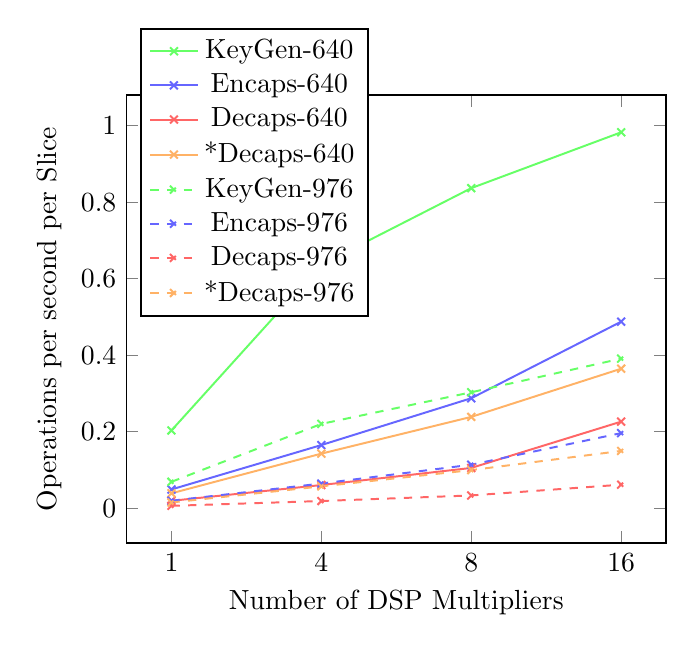
\begin{tikzpicture}
	\begin{axis}[
		xlabel=Number of DSP Multipliers,
		ylabel=Operations per second per Slice,
		line width=0.25mm,
		xtick={0,1,2,3},
		xticklabels={1,4,8,16},
		legend style={at={(0.45,1.15)}}
]
	\addplot[color=green!60,mark=x] coordinates {
		(0,0.203448275862069)	
		(1,0.636619718309859)
		(2,0.836466165413534)
		(3,0.982456140350877)
	};
	\addplot[color=blue!60,mark=x] coordinates {
		(0,0.049152542372881)
		(1,0.165171898355755)
		(2,0.287542087542088)
		(3,0.48758865248227)
	};
	\addplot[color=red!60,mark=x] coordinates {
		(0,0.019434026593931)
		(1,0.060747663551402)
		(2,0.105390835579515)
		(3,0.22636815920398)
	};
	\addplot[color=orange!60,mark=x] coordinates {
		(0,0.039074960127592)
		(1,0.14275092936803)
		(2,0.238767650834403)
		(3,0.364663585002568)
	};
	\addplot[color=green!60,mark=x,dashed] coordinates {
		(0,0.069060773480663)	
		(1,0.220454545454545)
		(2,0.303079416531604)
		(3,0.390969162995595)
	};
	\addplot[color=blue!60,mark=x,dashed] coordinates {
		(0,0.019654088050315)
		(1,0.064604810996564)
		(2,0.113805970149254)
		(3,0.196408529741863)
	};
	\addplot[color=red!60,mark=x,dashed] coordinates {
		(0,0.006319514661274)
		(1,0.018932874354561)
		(2,0.033500501504514)
		(3,0.061623056503603)
	};
	\addplot[color=orange!60,mark=x,dashed] coordinates {
		(0,0.015107913669065)
		(1,0.057241379310345)
		(2,0.09969040247678)
		(3,0.149853085210578)
	};
    \legend{KeyGen-640,Encaps-640,Decaps-640,*Decaps-640,KeyGen-976,Encaps-976,Decaps-976,*Decaps-976}
	\end{axis}
\end{tikzpicture}
}
\caption{Comparison of the throughput performance per FPGA slice on a Xilinx Artix-7.}
 \label{fig:hw_line}
\end{figure}
\vspace{-0.2cm}
\section{Conclusions}\label{sec:conclusions}

The main contributions of this research is to evaluate the lattice-based KEM and potential NIST post-quantum standard, FrodoKEM \cite{frodokem}, in hardware. We develop designs which can reach up to 825 operations per second, where most of the designs fit in under 1500 slices. Area consumption results are less than the previous state-of-the-art, and are much lower than many of the other post-quantum hardware designs shown in Table \ref{tab:pqc}. We significantly improve the throughput performance compared to the state-of-the-art, by increasing the number of parallel multipliers we use during matrix multiplication. In order to do this efficiently, we replace an inefficient PRNG previously used, cSHAKE, with a much faster and smaller PRNG, Trivium. As a result, we are able to obtain either a much lower FPGA footprint (up to 5x smaller) or a much higher throughput (up to 16x faster) compared to previous research. Our implementations run in constant computational time and the designs comply with the Round 2 version of FrodoKEM in all aspects except for this PRNG choice. To further evaluate the performance of FrodoKEM, we implemented first-order masking for decapsulation, and we showed that it can be achieved with almost no effect on performance.

The results show that FrodoKEM is an ideal candidate for hardware designs, showing potential for high-throughput performances whilst still maintaining relatively small FPGA area consumption. Moreover, compared to other NIST lattice-based candidates, it has a lot more flexibility, such as increasing throughput without completely re-designing the multiplication component, compared to, for example, a NTT multiplier.

 
%%%%%%%%%%%%%%%%%%%%%%%%%%%%%%%%%%%%%%%%%%%%%%%%%%%%%%%%%%%%%%%%%%%%%%%%%%%%%%%
\bibliographystyle{splncs04}
\bibliography{bibliography}

\end{document}
